\section{Recurrent Neural Networks}


\begin{frame}
	\frametitle{The Recurrent Neural Network Hypothesis Space}
	The \alert{recurrent neural network (RNN)} architecture
	% \setlength{\leftmargini}{0.5em}
	\begin{columns}
		\begin{column}[T, onlytextwidth]{.45\textwidth}%
		\setlength{\partopsep}{0pt}%
		\begin{equation*}
			\begin{aligned}
			h_{k+1} &= \sigma(Wh_{k} + Ux_{k}),
			\qquad h_k \in \R^m
			% \qquad k=0,1,\dots,K-1
			\\
			h_0 &= 0
			\\
			\wh{y}_k &= c^\tp h_{k}
			\end{aligned}
		\end{equation*}
		\end{column}%
		\begin{column}[T]{.45\textwidth}
		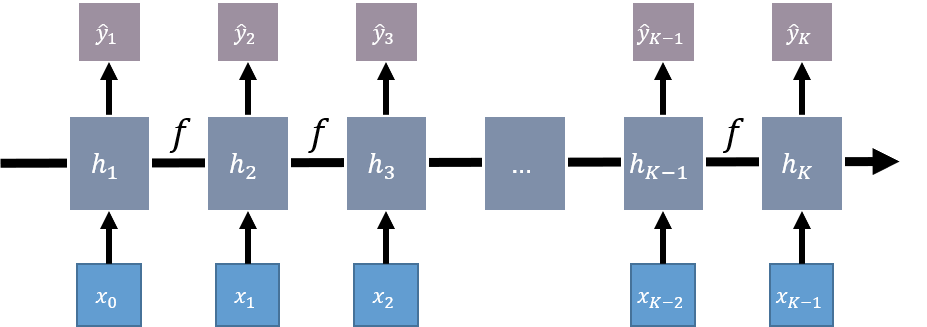
\includegraphics[width=\textwidth]{figures/recurrent_structure.png}
		\end{column}%
	\end{columns}

	\vspace{.5cm}

	\pause{}


    \begin{itemize}[<+->]
        \item
        The RNN parametrizes a sequence of functions
        $
            \{
            \wh{H}_k
            =
            \{x_0,\dots,x_{k-1}\} \mapsto \wh{y}_k
            \}.
        $
        \item
        A continuous-time idealization parametrizes functionals
        $\{ \*x \equiv \{x_t\} \mapsto \wh{y}_t \}$
        \begin{equation*}
            \dot{h}_t = \sigma(Wh_t + Ux_t),
            \quad h_{-\infty} = 0,
            \quad \wh{y}_t = c^\tp h_t,
            \quad t \in \R
        \end{equation*}
        \item
        Note: this is different from the dynamical viewpoint on deep neural networks,
        where the considered mapping is the flow map $h_0 \mapsto h_T$ \refhl{[E, 2017]}.
        Approximation theory: \refhl{[LLS, 2022]}

    \end{itemize}

    {\only<4->{
            \blfootnote{
                \fullcite{li2022deep}
            }
        }
    }
\end{frame}

\begin{frame}[focus]
    Empirically, it is found RNN performs poorly when modelling \\
	``long-term memory''

    \medskip

    Can we investigate this phenomena precisely?
\end{frame}


\begin{frame}
    \frametitle{The Linear RNN Hypothesis Space}

	We analyze the linear case where $\sigma(h) = h$, we have the dynamics
    \begin{equation*}
        \begin{split}
            \begin{aligned}
                \wh{y}_t &= c^\top h_t, \\
                \dot{h}_t &= W h_t + U x_t.
            \end{aligned}
        \end{split}
        \qquad
        \text{where}
        \qquad
        \begin{split}
            \begin{aligned}
                &h_t \in \R^m
                & & \text{(hidden state)}
                \\
                &W \in \R^{m \times m}
                & & \text{(Recurrent Kernel)}
                \\
                &U \in \R^{m \times d}
                & & \text{(Input Kernel)} \\
                &c \in \R^{m}
                & & \text{(Output layer weights)}
            \end{aligned}
        \end{split}
    \end{equation*}

    \pause{}

    This gives rise to the (stable) linear RNN hypothesis space

	\small
    \begin{empheq}[box=\mymath]{gather*}
        \hrnn =
        \cup_{m\geq 1}
        \underbrace{
            \left\{
                \{\wh{H}_t(\*x), t\in\R \} : \wh{H}_t(\*x) = \int_{0}^{\infty} c^\tp e^{Ws} U x_{t-s} ds,
                W \in \Wcal_m, U\in\R^{m\times d}, c \in \R^{m}
            \right\}
        }_{\hrnn^{(m)}}\\
        \Wcal_m = \{ W \in \R^{m\times m} : \text{eigenvalues of $W$ have negative real parts (Hurwitz)} \}
    \end{empheq}
	\normalsize
\end{frame}

\begin{frame}
    \frametitle{Properties of Linear RNN Hypothesis Space}

    \begin{empheq}[box=\mymath]{gather*}
        \hrnn^{(m)} =
        \cup_{m\geq 1}
		\left\{
			\{ \wh{H}_t(\*x) = \int_{0}^{\infty} c^\tp e^{Ws} U x_{t-s} ds \}
			:
			W \in \Wcal_m, U\in\R^{m\times d}, c \in \R^{m}
		\right\}
    \end{empheq}

    \begin{alertblock}{Proposition}
        Let $\{ \wh{H}_t : t\in\R \}$ be any family of functionals in $\hrnn$.
        Then for each $t\in\R$,
        \begin{itemize}
            \item $\wh{H}_t$ is a continuous, linear functional.
            \item $\wh{H}_t$ is a causal functional.
            \item $\wh{H}_t$ is a regular functional.
            \item The family $\{ \wh{H}_t : t\in\R\}$ is time-homogeneous.
        \end{itemize}
    \end{alertblock}

\end{frame}


\begin{frame}
	\frametitle{Approximation Guarantee (Density)}

	\begin{alertblock}{Theorem [LHEL, 2021]}
		Let $\{ \Htar_t : t\in\R \}$ be a family of continuous, linear, causal,
        regular and time-homogeneous functionals on $C_0(\R,\R^d)$.
        Then, for any $\epsilon > 0$ there exists $\{ \wh{H}_t : t\in \R \} \in \hrnn$ such that
		\begin{equation*}
            \| {\bm H^*} - {\wh{\bm H}} \|
            \equiv
			\sup_{t\in\R}
			\sup_{\| \*x \|_C \leq 1}
			|
			\Htar_t(\*x) - \wh{H}_t(\*x)
			|
			\leq \epsilon.
		\end{equation*}
	\end{alertblock}

	Main idea: Prove a general Riesz representation
	\begin{equation*}
		H^*_t(\*x) =
		\int_{0}^{\infty}
        \rho(s)^\tp
		x_{t-s}
		ds
        \qquad
        \alert{
            \left[
                \text{Recall: }
                \wh{H}_t(\*x) = \int_{0}^{\infty} c^\tp e^{Ws} U x_{t-s} ds
            \right]
        }
	\end{equation*}
	Then, RNN approximation reduces to the $L^1$ approximation of $\rho(t)$ by $[c^\tp e^{Wt} U]^\tp$.

	\blfootnote{
		\fullcite{li2020onthe}
	}

\end{frame}


\begin{frame}
    \frametitle{Smoothness and Memory}

	Approximation rates depend on appropriate complexity measures

    \pause{}

    Key concepts: \alert{smoothness} and \alert{memory}

    \begin{figure}
        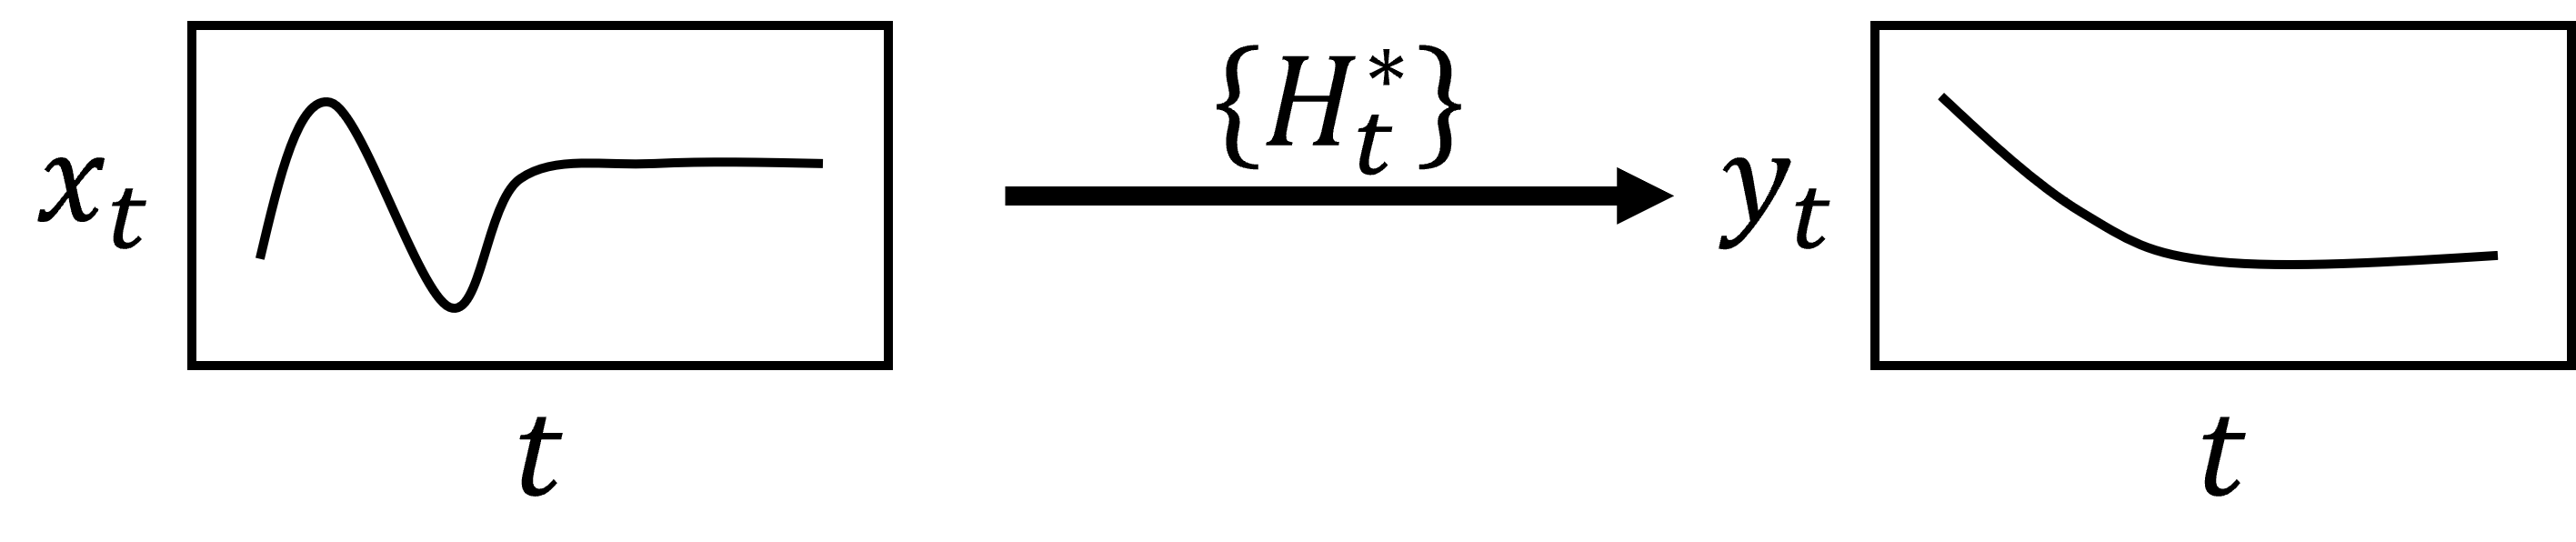
\includegraphics[width=0.48\textwidth]{figures/easy_approx.png}
        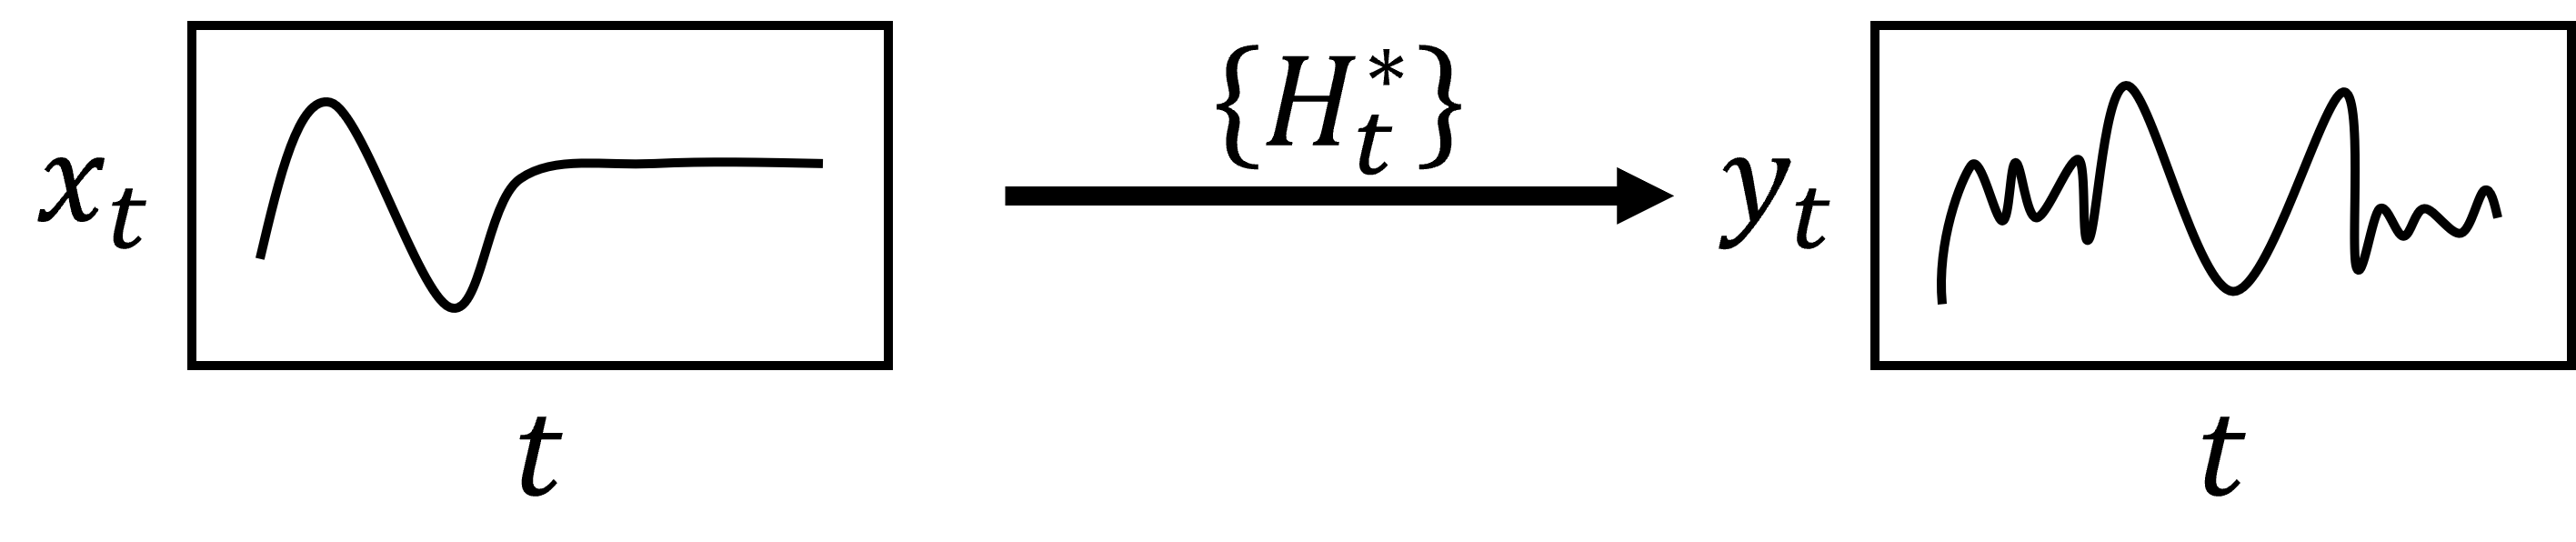
\includegraphics[width=0.48\textwidth]{figures/hard_approx.png}
    \end{figure}

    \pause{}

    Define
    \begin{itemize}
        \item $e_i$, $i=1,\dots,d$ as the standard basis vectors in $\R^d$
        \item $\*e_i$ as the constant signal $e_{i,t} = e_i \ind_{\{t\geq 0\}}$
    \end{itemize}

    \pause{}

    Given a family of functionals $\{\Htar_t : t\in\R\}$
    \begin{itemize}
        \item Denote the output of constant signal $y_i(t) := \Htar_t(\*e_i)$
        \item \alert{smoothness} is characterized by the smoothness of $t\mapsto y_i(t)$
        \item \alert{memory} is characterized by the decay rate of the $t\mapsto y_i^{(k)}(t)$
    \end{itemize}
\end{frame}


\begin{frame}
    \frametitle{Approximation Rate}

    \begin{alertblock}{Theorem [LHEL, 2021]}
        Set $y_i = H^*_t(\bm e_i)$.
        Suppose there exist constants $\alpha\in \Z^+, \beta,\gamma\in \R^+$
        such that for $i=1,\dots,d$, $y_i(t) \in C^{(\alpha+1)}(\R)$ and for $k=1,\dots,\alpha+1$,
        \begin{equation*}
            e^{\beta t}y_i^{(k)}(t) = o(1) \text{ as } t \rightarrow +\infty
            \qquad
            \text{and}
            \qquad
            \sup_{t \geq 0} \frac{ |e^{\beta t}y_i^{(k)}(t)|}{\beta^k} \leq \gamma.
        \end{equation*}
        Then there exists a universal constant $C(\alpha)$ such that for each $m \geq 1$,
        % there exists $\{\wh{H}_t\} \in \wh{\Hcal}_m$ such that
        \begin{equation*}
            \inf_{\wh{\bm H} \in \hrnn^{(m)}}
            \| \bm \Htar - \wh{\bm H} \|
            % \sup_{t\in\R}
            % \| \Htar_t - \wh{H}_t \|
            % \equiv
            % \sup_{t\in\R}
            % \sup_{\| \*x \|_C \leq 1}
            % |
            %     \Htar_t(\*x) - \wh{H}_t(\*x)
            % |
            \leq \frac{C(\alpha)\gamma d}{ \beta m^\alpha}.
        \end{equation*}
    \end{alertblock}

    \blfootnote{
        \fullcite{li2020onthe}
    }
\end{frame}

\begin{frame}
	\frametitle{Curse of Memory in Approximation}

    Rate estimate
    \begin{equation*}
        \inf_{\wh{\bm H} \in \hrnn^{(m)}}
        \| \bm \Htar - \wh{\bm H} \|
        % \sup_{t\in\R}
        % \|
        %     H^*_t - \wh{H}_t
        % \|
        \leq \frac{C(\alpha)\gamma d}{ \beta m^\alpha}.
    \end{equation*}

    \pause{}

    Observations
    \begin{itemize}[<+->]
        \item The smoothness dependence ($\alpha$) is what one would expect in approximation theory
        \item The memory dependence ($\beta,\gamma$) is new:
        assumption means the temporal derivatives of
        $y_i(t) \equiv \Htar_t(\*e_i)$ must decay like $e^{-\beta t}$ for some $\beta>0$
        \item There is no curse of dimensionality - this is because we are in a linear setting,
        so dimensions can be separated in a linear fashion
        \item However, hidden in these results is a \alert{curse of memory}.
        A truncation argument shows that
    \end{itemize}

    {\onslide<5>
        \begin{empheq}[box=\mymath]{align*}
            \text{If $H^*_t(\*e_i) \sim t^{-\omega}$},
            \text{ then to get error $\epsilon$, need }
            m \sim
            \mathcal{O}
            \left(
                \omega \varepsilon^{-\frac{1}{\omega}}
            \right)
        \end{empheq}
    }
\end{frame}

\begin{frame}
	\frametitle{Insights on the (Linear) RNN Hypothesis Space}

    \begin{empheq}[box=\mymath]{gather*}
        \text{
            \textbf{Insight:}
            Efficient approximation if ${\bm H^*}$ is smooth
        } \\
		\text{
			and has exponential decaying memory
		}
    \end{empheq}

	Futhermore
	\begin{itemize}
		\item The ``only if'' part is also true \refhl{[LHEL, 2022]}
		\begin{equation*}
			\text{efficient approximation}
			\quad \implies \quad
			\text{exponential decaying memory}
		\end{equation*}
		\item A related curse of memory holds for optimizing RNNs \refhl{[LHEL, 2021; 2022]}
	\end{itemize}

    \blfootnote{
        \fullcite{li2020onthe}
    }
    \blfootnote{
        \fullcite{li2022approxlinear}
    }
\end{frame}